\subsection{Sicherheitsmodell nach Gordon Cooper}\label{ss:Sicherheitsmodell}


Wie schützt man das \ac{IoT}?\\

Um diese Frage beantworten zu können, müssen die Schnittstellen und Eckpunkte des \ac{IoT}s definiert werden, welche Hackern Angriffsflächen bieten. Zu diesem Zweck hat Gordon Cooper ein Sicherheitsmodell aufgestellt, anhand dessen Sicherheitsmaßnahmen erklärt werden können. Dieses Sicherheitsmodell wird in Abbildung ~\ref{f:security} dargestellt.

\vspace{5 mm}
\begin{figure}[H] 
	\centering
	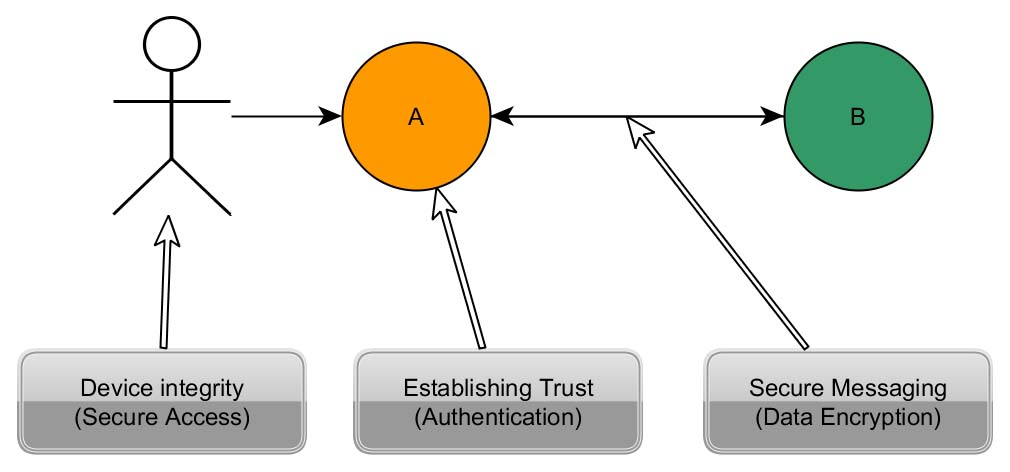
\includegraphics[scale=0.4]{Bilder/sicherheitsmodell}
	\caption{Sicherheitsmodell nach Gordon Cooper\cite{z:DesignElektronik}}
	\label{f:security}
\end{figure}
\vspace{5 mm}

Um die Integrität der \ac{IoT}-Komponenten zu schützen, muss der Zugang und somit die Anmeldung an jedem Knoten geschützt werden. Dies wird im Sicherheitsmodell nach Gordon Cooper als 'Secure Access' bezeichnet.\\
Wie auch im privaten Umfeld wird das Funknetz, in dem sich die Teilnehmer des \ac{IoT}s einklinken, durch einen Sicherheitsschlüssel geschützt. Dieser muss von den Geräten, sowie allen Benutzern angegeben werden, um Zugang zum Netz zu erhalten. Eine wichtige Aufgabe besteht darin, diesen Schlüssel zu schützen. Hierbei muss unter anderem die Weitergabe, sowie die Kommunikation im Netz durchdacht und überwacht werden. Besonders bei der Schlüsselwahl ist Vorsicht geboten. Es sollten niemals Namen, Geburtsdaten oder andere Informationen, die einer Person zugeordnet werden können, verwendet werden. Zusätzlich sind gebräuchliche Wörter nicht empfehlenswert, da diese leicht durch Wörterbuchangriffe überlistet werden können. Damit die Sicherheit des Passworts gewährleistet ist, sollte es mindestens 8 Zeichen enthalten und Groß-/Kleinschreibung, sowie Sonderzeichen und Zahlen enthalten. Eine allgemeingültige Faustregel ist: Je länger, desto besser.\\

Eine weitere Sicherheitsmaßnahme sind maßgeschneiderte Zugriffsrechte. Jeder Teilnehmer im \ac{IoT} darf nur so viele Rechte besitzen, wie unbedingt nötig. Hierdurch wird sichergestellt, dass Angreifer beim Erlangen eines Zugangscodes nur eingeschränkte Handlungsmöglichkeiten besitzen und der mögliche Schaden gering gehalten wird.\\

Um die Anmeldung an \ac{IoT}-Geräten möglichst sicher zu gestalten, sollte ein asymmetrisches Schlüsselpaar verwendet werden. Hierbei wird pro Kommunikationsteilnehmer ein Schlüsselpaar verwendet, das aus einem öffentlichen Schlüssel, dem 'Public Key' und einem privaten Schlüssel, dem 'Private Key' besteht. Wie der Name bereits sagt, ist der 'Private Key' nur beim Schlüsselinhaber vorzufinden und darf nicht öffentlich werden. Der 'Public Key' hingegen wird jedem Kommunikationspartner bereitgestellt und kann über unsichere Kommunikationswege geteilt werden.\\

Die Verschlüsselung der Kommunikation geschieht mit einem Algorithmus, der das Entschlüsseln nur mit dem nicht zum Verschlüsseln verwendeten Schlüssel ermöglicht. Dies bedeutet, dass von dem Inhaber des 'Private Keys' versendete Nachrichten auch unbestreitbar von ihm stammen. Durch die hiermit stattfindende Authentifikation wird der zweite Sektor 'Authentication' des Sicherheitsmodells nach Gordon Cooper erfüllt.

Da jede Kommunikation zwischen zwei \ac{IoT}-Komponenten potentiell sensible Daten beinhalten kann, muss permanent ein verschlüsselter Kanal verwendet werden. Dies ist im Sicherheitsmodell mit dem Sektor 'Secure Messaging - Data Encryption' beschrieben. Um dies effizient zu gestalten, wird das beschriebene Public-Key-Verfahren genutzt, um einen symmetrischen Schlüssel auszuhandeln. Bei diesem handelt es sich um einen Schlüssel, der sowohl zum Ver- als auch Entschlüsseln verwendet wird. Dieser Sitzungsschlüssel, genannt 'Session-Key', wird bei der Kommunikationsaufnahme der Komponenten generiert und mit Hilfe des 'Public-Keys' des Kommunikationspartners verschlüsselt. Daraufhin ist es dem Empfänger möglich, den symmetrischen Schlüssel für die weitere Kommunikation zu verwenden. Da der Session-Key bei jeder Sitzung neu ausgehandelt wird, ist er nur den Kommunikationspartnern bekannt und bietet ausreichende Sicherheit.\\